% !TEX root = hazelnut-popl17.tex
\subsection{Implementation Concepts}
Central to any implementation of Hazelnut is a stream of edit states whose cursor erasures synthesize types under an empty context according to the synthetic action judgement, $\performSyn{\emptyset}{\zexp}{\htau}{\alpha}{\zexp'}{\htau'}$. The middle row of Figure \ref{fig:impl-overview} diagrams this stream of edit states. By Theorem \ref{thrm:actsafe}, the editor does not need to typecheck each edit state (though in some of the rules, e.g. Rule (\ref{rule:zipper-asc}) which handles the situation where the type in a type ascription changes, portions of the program do need to be typechecked.) For example, the reader is encouraged to re-examine the examples in Figure \ref{fig:first-example} and \ref{fig:second-example} -- the cursor erasure of each edit state synthesizes a type.

The programmer examines a view generated from each edit state and produces actions in some implementation-defined manner (e.g. using a keyboard, mouse, touchscreen, voice interface, or neural implant.) Each new action causes a new abstract edit state to arise according to an implementation of the action semantics. This then causes a new view to arise. This is a simple event-based functional reactive programming model \cite{Wan:2000:FRP:349299.349331}. 

If an action is not well-defined according to Hazelnut's action semantics, the implementation must reject it. In fact, the implementation is encouraged to present an ``action palette'' that either hides or visibly disables actions that are not well-defined (see below.)



\begin{figure}
\centering
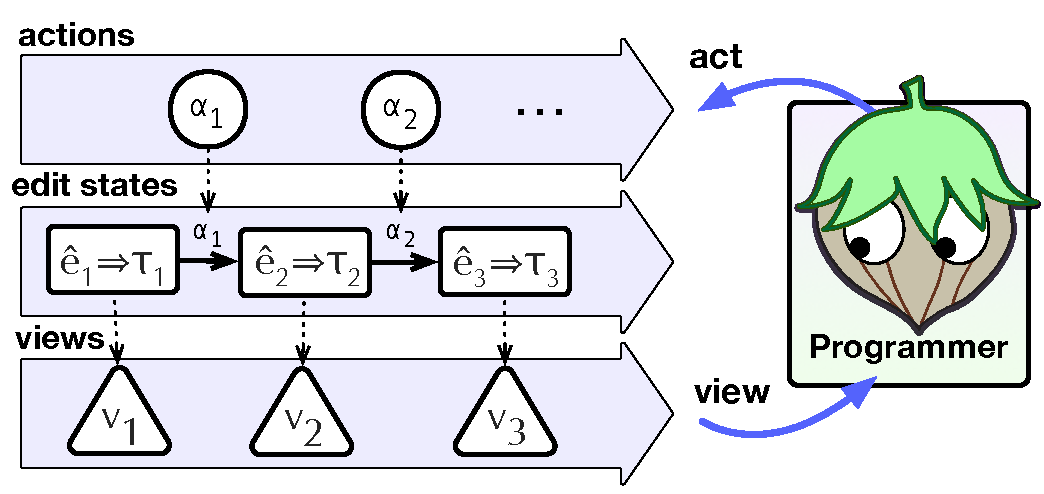
\includegraphics[width=\columnwidth]{impl-overview2}
\caption{Implementation Concepts}
\label{fig:impl-overview}
\end{figure}

\subsection{HZ}
We have developed a simple reference implementation, HZ, of Hazelnut.
In order to reach a wide audience, we decided to implement HZ in the web browser.
In order to take advantage of a mature implementation of the FRP model, we chose to implement HZ using OCaml\footnote{\url{https://ocaml.org/}}, the \texttt{js\_of\_ocaml} compiler and associated libraries \cite{DBLP:conf/ml/Balat06}\footnote{\url{http://ocsigen.org/js\_of\_ocaml/}} and the OCaml React library\footnote{\url{http://erratique.ch/software/react}}.

At the time of the writing, 
HZ's view computation renders the model as a string embedded into HTML that approximates our typeset notation in this paper. The action palette is a collection of buttons and text boxes, which are disabled when an action is not well-defined or an invalid action argument is entered. We determine this by simply attempting to perform the action internally and catching the exception that is raised when an action is undefined. This design, of course, is not meant to score marks for usability or performance. Instead, as a simple reference implementation, we expect its source code to be of use to others who are interested in layering a more fluid user interface atop the core semantics (which have been implemented in a style that follows the presentation in this paper closely), or extensions thereof.
